% Created by tikzDevice version 0.8.1 on 2015-05-16 17:35:04
% !TEX encoding = UTF-8 Unicode
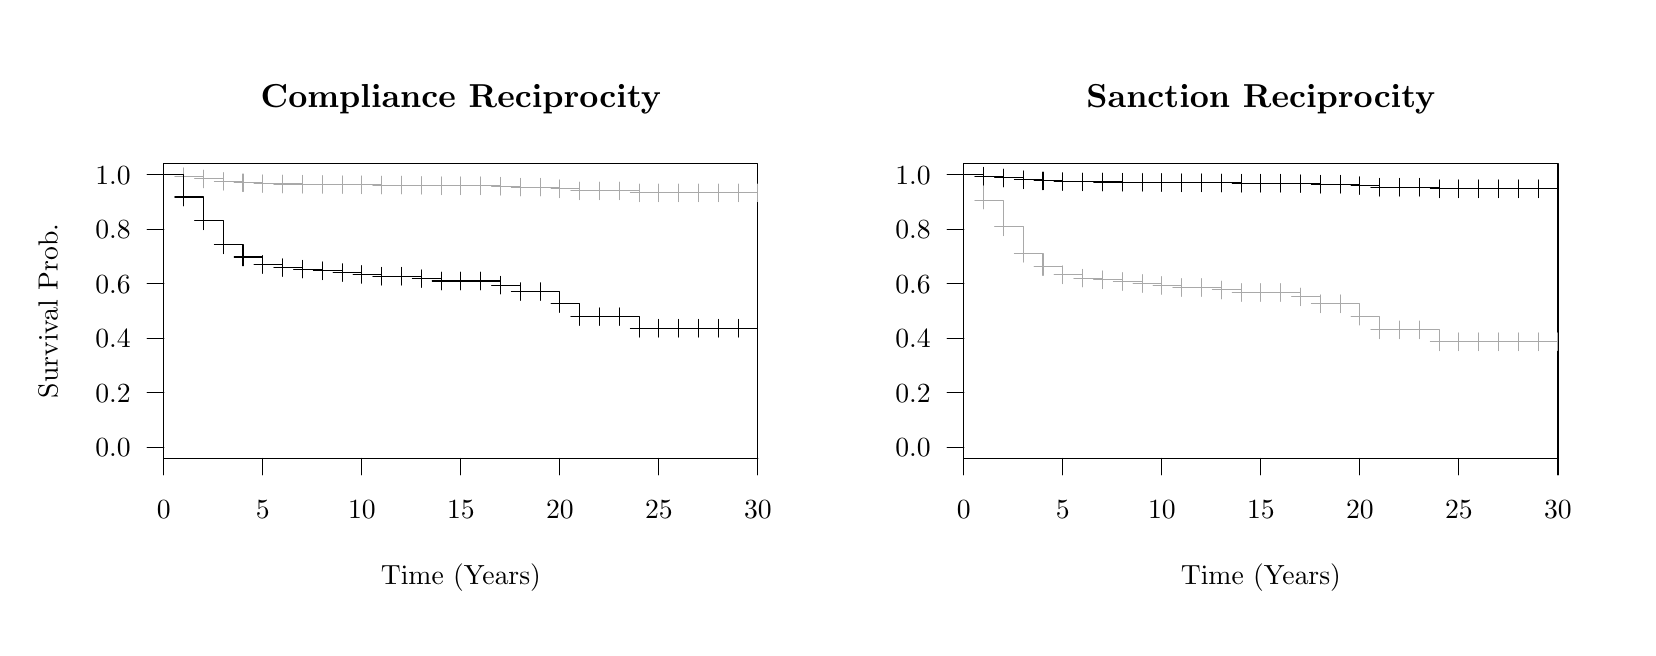
\begin{tikzpicture}[x=1pt,y=1pt]
\definecolor{fillColor}{RGB}{255,255,255}
\path[use as bounding box,fill=fillColor,fill opacity=0.00] (0,0) rectangle (578.16,216.81);
\begin{scope}
\path[clip] (  0.00,  0.00) rectangle (578.16,216.81);
\definecolor{drawColor}{RGB}{0,0,0}

\path[draw=drawColor,line width= 0.4pt,line join=round,line cap=round] ( 49.20, 61.20) -- (263.88, 61.20);

\path[draw=drawColor,line width= 0.4pt,line join=round,line cap=round] ( 49.20, 61.20) -- ( 49.20, 55.20);

\path[draw=drawColor,line width= 0.4pt,line join=round,line cap=round] ( 84.98, 61.20) -- ( 84.98, 55.20);

\path[draw=drawColor,line width= 0.4pt,line join=round,line cap=round] (120.76, 61.20) -- (120.76, 55.20);

\path[draw=drawColor,line width= 0.4pt,line join=round,line cap=round] (156.54, 61.20) -- (156.54, 55.20);

\path[draw=drawColor,line width= 0.4pt,line join=round,line cap=round] (192.32, 61.20) -- (192.32, 55.20);

\path[draw=drawColor,line width= 0.4pt,line join=round,line cap=round] (228.10, 61.20) -- (228.10, 55.20);

\path[draw=drawColor,line width= 0.4pt,line join=round,line cap=round] (263.88, 61.20) -- (263.88, 55.20);

\node[text=drawColor,anchor=base,inner sep=0pt, outer sep=0pt, scale=  1.00] at ( 49.20, 39.60) {0};

\node[text=drawColor,anchor=base,inner sep=0pt, outer sep=0pt, scale=  1.00] at ( 84.98, 39.60) {5};

\node[text=drawColor,anchor=base,inner sep=0pt, outer sep=0pt, scale=  1.00] at (120.76, 39.60) {10};

\node[text=drawColor,anchor=base,inner sep=0pt, outer sep=0pt, scale=  1.00] at (156.54, 39.60) {15};

\node[text=drawColor,anchor=base,inner sep=0pt, outer sep=0pt, scale=  1.00] at (192.32, 39.60) {20};

\node[text=drawColor,anchor=base,inner sep=0pt, outer sep=0pt, scale=  1.00] at (228.10, 39.60) {25};

\node[text=drawColor,anchor=base,inner sep=0pt, outer sep=0pt, scale=  1.00] at (263.88, 39.60) {30};

\path[draw=drawColor,line width= 0.4pt,line join=round,line cap=round] ( 49.20, 65.14) -- ( 49.20,163.67);

\path[draw=drawColor,line width= 0.4pt,line join=round,line cap=round] ( 49.20, 65.14) -- ( 43.20, 65.14);

\path[draw=drawColor,line width= 0.4pt,line join=round,line cap=round] ( 49.20, 84.85) -- ( 43.20, 84.85);

\path[draw=drawColor,line width= 0.4pt,line join=round,line cap=round] ( 49.20,104.55) -- ( 43.20,104.55);

\path[draw=drawColor,line width= 0.4pt,line join=round,line cap=round] ( 49.20,124.26) -- ( 43.20,124.26);

\path[draw=drawColor,line width= 0.4pt,line join=round,line cap=round] ( 49.20,143.96) -- ( 43.20,143.96);

\path[draw=drawColor,line width= 0.4pt,line join=round,line cap=round] ( 49.20,163.67) -- ( 43.20,163.67);

\node[text=drawColor,anchor=base east,inner sep=0pt, outer sep=0pt, scale=  1.00] at ( 37.20, 61.70) {0.0};

\node[text=drawColor,anchor=base east,inner sep=0pt, outer sep=0pt, scale=  1.00] at ( 37.20, 81.40) {0.2};

\node[text=drawColor,anchor=base east,inner sep=0pt, outer sep=0pt, scale=  1.00] at ( 37.20,101.11) {0.4};

\node[text=drawColor,anchor=base east,inner sep=0pt, outer sep=0pt, scale=  1.00] at ( 37.20,120.81) {0.6};

\node[text=drawColor,anchor=base east,inner sep=0pt, outer sep=0pt, scale=  1.00] at ( 37.20,140.52) {0.8};

\node[text=drawColor,anchor=base east,inner sep=0pt, outer sep=0pt, scale=  1.00] at ( 37.20,160.23) {1.0};

\path[draw=drawColor,line width= 0.4pt,line join=round,line cap=round] ( 49.20, 61.20) --
	(263.88, 61.20) --
	(263.88,167.61) --
	( 49.20,167.61) --
	( 49.20, 61.20);
\end{scope}
\begin{scope}
\path[clip] (  0.00,  0.00) rectangle (289.08,216.81);
\definecolor{drawColor}{RGB}{0,0,0}

\node[text=drawColor,anchor=base,inner sep=0pt, outer sep=0pt, scale=  1.20] at (156.54,188.07) {\bfseries Compliance Reciprocity};
\end{scope}
\begin{scope}
\path[clip] ( 49.20, 61.20) rectangle (263.88,167.61);
\definecolor{drawColor}{RGB}{169,169,169}

\path[draw=drawColor,line width= 0.4pt,line join=round,line cap=round] ( 49.20,163.67) --
	( 56.36,163.67) --
	( 56.36,162.97) --
	( 63.51,162.97) --
	( 63.51,162.16) --
	( 70.67,162.16) --
	( 70.67,161.27) --
	( 77.82,161.27) --
	( 77.82,160.77) --
	( 84.98,160.77) --
	( 84.98,160.45) --
	( 92.14,160.45) --
	( 92.14,160.32) --
	( 99.29,160.32) --
	( 99.29,160.25) --
	(106.45,160.25) --
	(106.45,160.18) --
	(113.60,160.18) --
	(113.60,160.10) --
	(120.76,160.10) --
	(120.76,160.01) --
	(127.92,160.01) --
	(127.92,159.92) --
	(142.23,159.92) --
	(142.23,159.82) --
	(149.38,159.82) --
	(149.38,159.70) --
	(170.85,159.70) --
	(170.85,159.51) --
	(178.01,159.51) --
	(178.01,159.19) --
	(192.32,159.19) --
	(192.32,158.57) --
	(199.48,158.57) --
	(199.48,157.83) --
	(220.94,157.83) --
	(220.94,157.12) --
	(492.87,157.12) --
	(492.87,157.12);

\path[draw=drawColor,line width= 0.4pt,line join=round,line cap=round] ( 53.17,162.97) -- ( 59.54,162.97);

\path[draw=drawColor,line width= 0.4pt,line join=round,line cap=round] ( 56.36,159.79) -- ( 56.36,166.16);

\path[draw=drawColor,line width= 0.4pt,line join=round,line cap=round] ( 60.33,162.16) -- ( 66.69,162.16);

\path[draw=drawColor,line width= 0.4pt,line join=round,line cap=round] ( 63.51,158.98) -- ( 63.51,165.35);

\path[draw=drawColor,line width= 0.4pt,line join=round,line cap=round] ( 67.49,161.27) -- ( 73.85,161.27);

\path[draw=drawColor,line width= 0.4pt,line join=round,line cap=round] ( 70.67,158.09) -- ( 70.67,164.45);

\path[draw=drawColor,line width= 0.4pt,line join=round,line cap=round] ( 74.64,160.77) -- ( 81.01,160.77);

\path[draw=drawColor,line width= 0.4pt,line join=round,line cap=round] ( 77.82,157.59) -- ( 77.82,163.96);

\path[draw=drawColor,line width= 0.4pt,line join=round,line cap=round] ( 81.80,160.45) -- ( 88.16,160.45);

\path[draw=drawColor,line width= 0.4pt,line join=round,line cap=round] ( 84.98,157.27) -- ( 84.98,163.64);

\path[draw=drawColor,line width= 0.4pt,line join=round,line cap=round] ( 88.95,160.32) -- ( 95.32,160.32);

\path[draw=drawColor,line width= 0.4pt,line join=round,line cap=round] ( 92.14,157.13) -- ( 92.14,163.50);

\path[draw=drawColor,line width= 0.4pt,line join=round,line cap=round] ( 96.11,160.25) -- (102.47,160.25);

\path[draw=drawColor,line width= 0.4pt,line join=round,line cap=round] ( 99.29,157.07) -- ( 99.29,163.43);

\path[draw=drawColor,line width= 0.4pt,line join=round,line cap=round] (103.27,160.18) -- (109.63,160.18);

\path[draw=drawColor,line width= 0.4pt,line join=round,line cap=round] (106.45,156.99) -- (106.45,163.36);

\path[draw=drawColor,line width= 0.4pt,line join=round,line cap=round] (110.42,160.10) -- (116.79,160.10);

\path[draw=drawColor,line width= 0.4pt,line join=round,line cap=round] (113.60,156.91) -- (113.60,163.28);

\path[draw=drawColor,line width= 0.4pt,line join=round,line cap=round] (117.58,160.01) -- (123.94,160.01);

\path[draw=drawColor,line width= 0.4pt,line join=round,line cap=round] (120.76,156.83) -- (120.76,163.20);

\path[draw=drawColor,line width= 0.4pt,line join=round,line cap=round] (124.73,159.92) -- (131.10,159.92);

\path[draw=drawColor,line width= 0.4pt,line join=round,line cap=round] (127.92,156.74) -- (127.92,163.11);

\path[draw=drawColor,line width= 0.4pt,line join=round,line cap=round] (131.89,159.92) -- (138.25,159.92);

\path[draw=drawColor,line width= 0.4pt,line join=round,line cap=round] (135.07,156.74) -- (135.07,163.11);

\path[draw=drawColor,line width= 0.4pt,line join=round,line cap=round] (139.05,159.82) -- (145.41,159.82);

\path[draw=drawColor,line width= 0.4pt,line join=round,line cap=round] (142.23,156.64) -- (142.23,163.00);

\path[draw=drawColor,line width= 0.4pt,line join=round,line cap=round] (146.20,159.70) -- (152.57,159.70);

\path[draw=drawColor,line width= 0.4pt,line join=round,line cap=round] (149.38,156.52) -- (149.38,162.89);

\path[draw=drawColor,line width= 0.4pt,line join=round,line cap=round] (153.36,159.70) -- (159.72,159.70);

\path[draw=drawColor,line width= 0.4pt,line join=round,line cap=round] (156.54,156.52) -- (156.54,162.89);

\path[draw=drawColor,line width= 0.4pt,line join=round,line cap=round] (160.51,159.70) -- (166.88,159.70);

\path[draw=drawColor,line width= 0.4pt,line join=round,line cap=round] (163.70,156.52) -- (163.70,162.89);

\path[draw=drawColor,line width= 0.4pt,line join=round,line cap=round] (167.67,159.51) -- (174.03,159.51);

\path[draw=drawColor,line width= 0.4pt,line join=round,line cap=round] (170.85,156.33) -- (170.85,162.69);

\path[draw=drawColor,line width= 0.4pt,line join=round,line cap=round] (174.83,159.19) -- (181.19,159.19);

\path[draw=drawColor,line width= 0.4pt,line join=round,line cap=round] (178.01,156.01) -- (178.01,162.37);

\path[draw=drawColor,line width= 0.4pt,line join=round,line cap=round] (181.98,159.19) -- (188.35,159.19);

\path[draw=drawColor,line width= 0.4pt,line join=round,line cap=round] (185.16,156.01) -- (185.16,162.37);

\path[draw=drawColor,line width= 0.4pt,line join=round,line cap=round] (189.14,158.57) -- (195.50,158.57);

\path[draw=drawColor,line width= 0.4pt,line join=round,line cap=round] (192.32,155.39) -- (192.32,161.76);

\path[draw=drawColor,line width= 0.4pt,line join=round,line cap=round] (196.29,157.83) -- (202.66,157.83);

\path[draw=drawColor,line width= 0.4pt,line join=round,line cap=round] (199.48,154.65) -- (199.48,161.01);

\path[draw=drawColor,line width= 0.4pt,line join=round,line cap=round] (203.45,157.83) -- (209.81,157.83);

\path[draw=drawColor,line width= 0.4pt,line join=round,line cap=round] (206.63,154.65) -- (206.63,161.01);

\path[draw=drawColor,line width= 0.4pt,line join=round,line cap=round] (210.61,157.83) -- (216.97,157.83);

\path[draw=drawColor,line width= 0.4pt,line join=round,line cap=round] (213.79,154.65) -- (213.79,161.01);

\path[draw=drawColor,line width= 0.4pt,line join=round,line cap=round] (217.76,157.12) -- (224.13,157.12);

\path[draw=drawColor,line width= 0.4pt,line join=round,line cap=round] (220.94,153.94) -- (220.94,160.30);

\path[draw=drawColor,line width= 0.4pt,line join=round,line cap=round] (224.92,157.12) -- (231.28,157.12);

\path[draw=drawColor,line width= 0.4pt,line join=round,line cap=round] (228.10,153.94) -- (228.10,160.30);

\path[draw=drawColor,line width= 0.4pt,line join=round,line cap=round] (232.07,157.12) -- (238.44,157.12);

\path[draw=drawColor,line width= 0.4pt,line join=round,line cap=round] (235.26,153.94) -- (235.26,160.30);

\path[draw=drawColor,line width= 0.4pt,line join=round,line cap=round] (239.23,157.12) -- (245.59,157.12);

\path[draw=drawColor,line width= 0.4pt,line join=round,line cap=round] (242.41,153.94) -- (242.41,160.30);

\path[draw=drawColor,line width= 0.4pt,line join=round,line cap=round] (246.39,157.12) -- (252.75,157.12);

\path[draw=drawColor,line width= 0.4pt,line join=round,line cap=round] (249.57,153.94) -- (249.57,160.30);

\path[draw=drawColor,line width= 0.4pt,line join=round,line cap=round] (253.54,157.12) -- (259.91,157.12);

\path[draw=drawColor,line width= 0.4pt,line join=round,line cap=round] (256.72,153.94) -- (256.72,160.30);

\path[draw=drawColor,line width= 0.4pt,line join=round,line cap=round] (260.70,157.12) -- (267.06,157.12);

\path[draw=drawColor,line width= 0.4pt,line join=round,line cap=round] (263.88,153.94) -- (263.88,160.30);

\path[draw=drawColor,line width= 0.4pt,line join=round,line cap=round] (267.85,157.12) -- (274.22,157.12);

\path[draw=drawColor,line width= 0.4pt,line join=round,line cap=round] (271.04,153.94) -- (271.04,160.30);

\path[draw=drawColor,line width= 0.4pt,line join=round,line cap=round] (275.01,157.12) -- (281.37,157.12);

\path[draw=drawColor,line width= 0.4pt,line join=round,line cap=round] (278.19,153.94) -- (278.19,160.30);

\path[draw=drawColor,line width= 0.4pt,line join=round,line cap=round] (282.17,157.12) -- (288.53,157.12);

\path[draw=drawColor,line width= 0.4pt,line join=round,line cap=round] (285.35,153.94) -- (285.35,160.30);

\path[draw=drawColor,line width= 0.4pt,line join=round,line cap=round] (289.32,157.12) -- (295.69,157.12);

\path[draw=drawColor,line width= 0.4pt,line join=round,line cap=round] (292.50,153.94) -- (292.50,160.30);

\path[draw=drawColor,line width= 0.4pt,line join=round,line cap=round] (296.48,157.12) -- (302.84,157.12);

\path[draw=drawColor,line width= 0.4pt,line join=round,line cap=round] (299.66,153.94) -- (299.66,160.30);

\path[draw=drawColor,line width= 0.4pt,line join=round,line cap=round] (303.63,157.12) -- (310.00,157.12);

\path[draw=drawColor,line width= 0.4pt,line join=round,line cap=round] (306.82,153.94) -- (306.82,160.30);

\path[draw=drawColor,line width= 0.4pt,line join=round,line cap=round] (310.79,157.12) -- (317.15,157.12);

\path[draw=drawColor,line width= 0.4pt,line join=round,line cap=round] (313.97,153.94) -- (313.97,160.30);

\path[draw=drawColor,line width= 0.4pt,line join=round,line cap=round] (317.95,157.12) -- (324.31,157.12);

\path[draw=drawColor,line width= 0.4pt,line join=round,line cap=round] (321.13,153.94) -- (321.13,160.30);

\path[draw=drawColor,line width= 0.4pt,line join=round,line cap=round] (325.10,157.12) -- (331.47,157.12);

\path[draw=drawColor,line width= 0.4pt,line join=round,line cap=round] (328.28,153.94) -- (328.28,160.30);

\path[draw=drawColor,line width= 0.4pt,line join=round,line cap=round] (332.26,157.12) -- (338.62,157.12);

\path[draw=drawColor,line width= 0.4pt,line join=round,line cap=round] (335.44,153.94) -- (335.44,160.30);

\path[draw=drawColor,line width= 0.4pt,line join=round,line cap=round] (339.41,157.12) -- (345.78,157.12);

\path[draw=drawColor,line width= 0.4pt,line join=round,line cap=round] (342.60,153.94) -- (342.60,160.30);

\path[draw=drawColor,line width= 0.4pt,line join=round,line cap=round] (346.57,157.12) -- (352.93,157.12);

\path[draw=drawColor,line width= 0.4pt,line join=round,line cap=round] (349.75,153.94) -- (349.75,160.30);

\path[draw=drawColor,line width= 0.4pt,line join=round,line cap=round] (353.73,157.12) -- (360.09,157.12);

\path[draw=drawColor,line width= 0.4pt,line join=round,line cap=round] (356.91,153.94) -- (356.91,160.30);

\path[draw=drawColor,line width= 0.4pt,line join=round,line cap=round] (360.88,157.12) -- (367.25,157.12);

\path[draw=drawColor,line width= 0.4pt,line join=round,line cap=round] (364.06,153.94) -- (364.06,160.30);

\path[draw=drawColor,line width= 0.4pt,line join=round,line cap=round] (368.04,157.12) -- (374.40,157.12);

\path[draw=drawColor,line width= 0.4pt,line join=round,line cap=round] (371.22,153.94) -- (371.22,160.30);

\path[draw=drawColor,line width= 0.4pt,line join=round,line cap=round] (375.19,157.12) -- (381.56,157.12);

\path[draw=drawColor,line width= 0.4pt,line join=round,line cap=round] (378.38,153.94) -- (378.38,160.30);

\path[draw=drawColor,line width= 0.4pt,line join=round,line cap=round] (382.35,157.12) -- (388.71,157.12);

\path[draw=drawColor,line width= 0.4pt,line join=round,line cap=round] (385.53,153.94) -- (385.53,160.30);

\path[draw=drawColor,line width= 0.4pt,line join=round,line cap=round] (389.51,157.12) -- (395.87,157.12);

\path[draw=drawColor,line width= 0.4pt,line join=round,line cap=round] (392.69,153.94) -- (392.69,160.30);

\path[draw=drawColor,line width= 0.4pt,line join=round,line cap=round] (396.66,157.12) -- (403.03,157.12);

\path[draw=drawColor,line width= 0.4pt,line join=round,line cap=round] (399.84,153.94) -- (399.84,160.30);

\path[draw=drawColor,line width= 0.4pt,line join=round,line cap=round] (403.82,157.12) -- (410.18,157.12);

\path[draw=drawColor,line width= 0.4pt,line join=round,line cap=round] (407.00,153.94) -- (407.00,160.30);

\path[draw=drawColor,line width= 0.4pt,line join=round,line cap=round] (410.97,157.12) -- (417.34,157.12);

\path[draw=drawColor,line width= 0.4pt,line join=round,line cap=round] (414.16,153.94) -- (414.16,160.30);

\path[draw=drawColor,line width= 0.4pt,line join=round,line cap=round] (418.13,157.12) -- (424.49,157.12);

\path[draw=drawColor,line width= 0.4pt,line join=round,line cap=round] (421.31,153.94) -- (421.31,160.30);

\path[draw=drawColor,line width= 0.4pt,line join=round,line cap=round] (425.29,157.12) -- (431.65,157.12);

\path[draw=drawColor,line width= 0.4pt,line join=round,line cap=round] (428.47,153.94) -- (428.47,160.30);

\path[draw=drawColor,line width= 0.4pt,line join=round,line cap=round] (432.44,157.12) -- (438.81,157.12);

\path[draw=drawColor,line width= 0.4pt,line join=round,line cap=round] (435.62,153.94) -- (435.62,160.30);

\path[draw=drawColor,line width= 0.4pt,line join=round,line cap=round] (439.60,157.12) -- (445.96,157.12);

\path[draw=drawColor,line width= 0.4pt,line join=round,line cap=round] (442.78,153.94) -- (442.78,160.30);

\path[draw=drawColor,line width= 0.4pt,line join=round,line cap=round] (446.75,157.12) -- (453.12,157.12);

\path[draw=drawColor,line width= 0.4pt,line join=round,line cap=round] (449.94,153.94) -- (449.94,160.30);

\path[draw=drawColor,line width= 0.4pt,line join=round,line cap=round] (453.91,157.12) -- (460.27,157.12);

\path[draw=drawColor,line width= 0.4pt,line join=round,line cap=round] (457.09,153.94) -- (457.09,160.30);

\path[draw=drawColor,line width= 0.4pt,line join=round,line cap=round] (461.07,157.12) -- (467.43,157.12);

\path[draw=drawColor,line width= 0.4pt,line join=round,line cap=round] (464.25,153.94) -- (464.25,160.30);

\path[draw=drawColor,line width= 0.4pt,line join=round,line cap=round] (468.22,157.12) -- (474.59,157.12);

\path[draw=drawColor,line width= 0.4pt,line join=round,line cap=round] (471.40,153.94) -- (471.40,160.30);

\path[draw=drawColor,line width= 0.4pt,line join=round,line cap=round] (475.38,157.12) -- (481.74,157.12);

\path[draw=drawColor,line width= 0.4pt,line join=round,line cap=round] (478.56,153.94) -- (478.56,160.30);

\path[draw=drawColor,line width= 0.4pt,line join=round,line cap=round] (482.53,157.12) -- (488.90,157.12);

\path[draw=drawColor,line width= 0.4pt,line join=round,line cap=round] (485.72,153.94) -- (485.72,160.30);

\path[draw=drawColor,line width= 0.4pt,line join=round,line cap=round] (489.69,157.12) -- (496.05,157.12);

\path[draw=drawColor,line width= 0.4pt,line join=round,line cap=round] (492.87,153.94) -- (492.87,160.30);
\definecolor{drawColor}{RGB}{0,0,0}

\path[draw=drawColor,line width= 0.4pt,line join=round,line cap=round] ( 49.20,163.67) --
	( 56.36,163.67) --
	( 56.36,155.62) --
	( 63.51,155.62) --
	( 63.51,147.01) --
	( 70.67,147.01) --
	( 70.67,138.40) --
	( 77.82,138.40) --
	( 77.82,133.95) --
	( 84.98,133.95) --
	( 84.98,131.24) --
	( 92.14,131.24) --
	( 92.14,130.11) --
	( 99.29,130.11) --
	( 99.29,129.56) --
	(106.45,129.56) --
	(106.45,128.96) --
	(113.60,128.96) --
	(113.60,128.31) --
	(120.76,128.31) --
	(120.76,127.66) --
	(127.92,127.66) --
	(127.92,126.96) --
	(142.23,126.96) --
	(142.23,126.13) --
	(149.38,126.13) --
	(149.38,125.25) --
	(170.85,125.25) --
	(170.85,123.77) --
	(178.01,123.77) --
	(178.01,121.43) --
	(192.32,121.43) --
	(192.32,117.16) --
	(199.48,117.16) --
	(199.48,112.39) --
	(220.94,112.39) --
	(220.94,108.19) --
	(492.87,108.19) --
	(492.87,108.19);

\path[draw=drawColor,line width= 0.4pt,line join=round,line cap=round] ( 53.17,155.62) -- ( 59.54,155.62);

\path[draw=drawColor,line width= 0.4pt,line join=round,line cap=round] ( 56.36,152.43) -- ( 56.36,158.80);

\path[draw=drawColor,line width= 0.4pt,line join=round,line cap=round] ( 60.33,147.01) -- ( 66.69,147.01);

\path[draw=drawColor,line width= 0.4pt,line join=round,line cap=round] ( 63.51,143.83) -- ( 63.51,150.19);

\path[draw=drawColor,line width= 0.4pt,line join=round,line cap=round] ( 67.49,138.40) -- ( 73.85,138.40);

\path[draw=drawColor,line width= 0.4pt,line join=round,line cap=round] ( 70.67,135.21) -- ( 70.67,141.58);

\path[draw=drawColor,line width= 0.4pt,line join=round,line cap=round] ( 74.64,133.95) -- ( 81.01,133.95);

\path[draw=drawColor,line width= 0.4pt,line join=round,line cap=round] ( 77.82,130.77) -- ( 77.82,137.14);

\path[draw=drawColor,line width= 0.4pt,line join=round,line cap=round] ( 81.80,131.24) -- ( 88.16,131.24);

\path[draw=drawColor,line width= 0.4pt,line join=round,line cap=round] ( 84.98,128.05) -- ( 84.98,134.42);

\path[draw=drawColor,line width= 0.4pt,line join=round,line cap=round] ( 88.95,130.11) -- ( 95.32,130.11);

\path[draw=drawColor,line width= 0.4pt,line join=round,line cap=round] ( 92.14,126.92) -- ( 92.14,133.29);

\path[draw=drawColor,line width= 0.4pt,line join=round,line cap=round] ( 96.11,129.56) -- (102.47,129.56);

\path[draw=drawColor,line width= 0.4pt,line join=round,line cap=round] ( 99.29,126.38) -- ( 99.29,132.74);

\path[draw=drawColor,line width= 0.4pt,line join=round,line cap=round] (103.27,128.96) -- (109.63,128.96);

\path[draw=drawColor,line width= 0.4pt,line join=round,line cap=round] (106.45,125.78) -- (106.45,132.15);

\path[draw=drawColor,line width= 0.4pt,line join=round,line cap=round] (110.42,128.31) -- (116.79,128.31);

\path[draw=drawColor,line width= 0.4pt,line join=round,line cap=round] (113.60,125.13) -- (113.60,131.49);

\path[draw=drawColor,line width= 0.4pt,line join=round,line cap=round] (117.58,127.66) -- (123.94,127.66);

\path[draw=drawColor,line width= 0.4pt,line join=round,line cap=round] (120.76,124.47) -- (120.76,130.84);

\path[draw=drawColor,line width= 0.4pt,line join=round,line cap=round] (124.73,126.96) -- (131.10,126.96);

\path[draw=drawColor,line width= 0.4pt,line join=round,line cap=round] (127.92,123.77) -- (127.92,130.14);

\path[draw=drawColor,line width= 0.4pt,line join=round,line cap=round] (131.89,126.96) -- (138.25,126.96);

\path[draw=drawColor,line width= 0.4pt,line join=round,line cap=round] (135.07,123.77) -- (135.07,130.14);

\path[draw=drawColor,line width= 0.4pt,line join=round,line cap=round] (139.05,126.13) -- (145.41,126.13);

\path[draw=drawColor,line width= 0.4pt,line join=round,line cap=round] (142.23,122.95) -- (142.23,129.31);

\path[draw=drawColor,line width= 0.4pt,line join=round,line cap=round] (146.20,125.25) -- (152.57,125.25);

\path[draw=drawColor,line width= 0.4pt,line join=round,line cap=round] (149.38,122.07) -- (149.38,128.44);

\path[draw=drawColor,line width= 0.4pt,line join=round,line cap=round] (153.36,125.25) -- (159.72,125.25);

\path[draw=drawColor,line width= 0.4pt,line join=round,line cap=round] (156.54,122.07) -- (156.54,128.44);

\path[draw=drawColor,line width= 0.4pt,line join=round,line cap=round] (160.51,125.25) -- (166.88,125.25);

\path[draw=drawColor,line width= 0.4pt,line join=round,line cap=round] (163.70,122.07) -- (163.70,128.44);

\path[draw=drawColor,line width= 0.4pt,line join=round,line cap=round] (167.67,123.77) -- (174.03,123.77);

\path[draw=drawColor,line width= 0.4pt,line join=round,line cap=round] (170.85,120.59) -- (170.85,126.95);

\path[draw=drawColor,line width= 0.4pt,line join=round,line cap=round] (174.83,121.43) -- (181.19,121.43);

\path[draw=drawColor,line width= 0.4pt,line join=round,line cap=round] (178.01,118.25) -- (178.01,124.62);

\path[draw=drawColor,line width= 0.4pt,line join=round,line cap=round] (181.98,121.43) -- (188.35,121.43);

\path[draw=drawColor,line width= 0.4pt,line join=round,line cap=round] (185.16,118.25) -- (185.16,124.62);

\path[draw=drawColor,line width= 0.4pt,line join=round,line cap=round] (189.14,117.16) -- (195.50,117.16);

\path[draw=drawColor,line width= 0.4pt,line join=round,line cap=round] (192.32,113.98) -- (192.32,120.34);

\path[draw=drawColor,line width= 0.4pt,line join=round,line cap=round] (196.29,112.39) -- (202.66,112.39);

\path[draw=drawColor,line width= 0.4pt,line join=round,line cap=round] (199.48,109.21) -- (199.48,115.57);

\path[draw=drawColor,line width= 0.4pt,line join=round,line cap=round] (203.45,112.39) -- (209.81,112.39);

\path[draw=drawColor,line width= 0.4pt,line join=round,line cap=round] (206.63,109.21) -- (206.63,115.57);

\path[draw=drawColor,line width= 0.4pt,line join=round,line cap=round] (210.61,112.39) -- (216.97,112.39);

\path[draw=drawColor,line width= 0.4pt,line join=round,line cap=round] (213.79,109.21) -- (213.79,115.57);

\path[draw=drawColor,line width= 0.4pt,line join=round,line cap=round] (217.76,108.19) -- (224.13,108.19);

\path[draw=drawColor,line width= 0.4pt,line join=round,line cap=round] (220.94,105.01) -- (220.94,111.38);

\path[draw=drawColor,line width= 0.4pt,line join=round,line cap=round] (224.92,108.19) -- (231.28,108.19);

\path[draw=drawColor,line width= 0.4pt,line join=round,line cap=round] (228.10,105.01) -- (228.10,111.38);

\path[draw=drawColor,line width= 0.4pt,line join=round,line cap=round] (232.07,108.19) -- (238.44,108.19);

\path[draw=drawColor,line width= 0.4pt,line join=round,line cap=round] (235.26,105.01) -- (235.26,111.38);

\path[draw=drawColor,line width= 0.4pt,line join=round,line cap=round] (239.23,108.19) -- (245.59,108.19);

\path[draw=drawColor,line width= 0.4pt,line join=round,line cap=round] (242.41,105.01) -- (242.41,111.38);

\path[draw=drawColor,line width= 0.4pt,line join=round,line cap=round] (246.39,108.19) -- (252.75,108.19);

\path[draw=drawColor,line width= 0.4pt,line join=round,line cap=round] (249.57,105.01) -- (249.57,111.38);

\path[draw=drawColor,line width= 0.4pt,line join=round,line cap=round] (253.54,108.19) -- (259.91,108.19);

\path[draw=drawColor,line width= 0.4pt,line join=round,line cap=round] (256.72,105.01) -- (256.72,111.38);

\path[draw=drawColor,line width= 0.4pt,line join=round,line cap=round] (260.70,108.19) -- (267.06,108.19);

\path[draw=drawColor,line width= 0.4pt,line join=round,line cap=round] (263.88,105.01) -- (263.88,111.38);

\path[draw=drawColor,line width= 0.4pt,line join=round,line cap=round] (267.85,108.19) -- (274.22,108.19);

\path[draw=drawColor,line width= 0.4pt,line join=round,line cap=round] (271.04,105.01) -- (271.04,111.38);

\path[draw=drawColor,line width= 0.4pt,line join=round,line cap=round] (275.01,108.19) -- (281.37,108.19);

\path[draw=drawColor,line width= 0.4pt,line join=round,line cap=round] (278.19,105.01) -- (278.19,111.38);

\path[draw=drawColor,line width= 0.4pt,line join=round,line cap=round] (282.17,108.19) -- (288.53,108.19);

\path[draw=drawColor,line width= 0.4pt,line join=round,line cap=round] (285.35,105.01) -- (285.35,111.38);

\path[draw=drawColor,line width= 0.4pt,line join=round,line cap=round] (289.32,108.19) -- (295.69,108.19);

\path[draw=drawColor,line width= 0.4pt,line join=round,line cap=round] (292.50,105.01) -- (292.50,111.38);

\path[draw=drawColor,line width= 0.4pt,line join=round,line cap=round] (296.48,108.19) -- (302.84,108.19);

\path[draw=drawColor,line width= 0.4pt,line join=round,line cap=round] (299.66,105.01) -- (299.66,111.38);

\path[draw=drawColor,line width= 0.4pt,line join=round,line cap=round] (303.63,108.19) -- (310.00,108.19);

\path[draw=drawColor,line width= 0.4pt,line join=round,line cap=round] (306.82,105.01) -- (306.82,111.38);

\path[draw=drawColor,line width= 0.4pt,line join=round,line cap=round] (310.79,108.19) -- (317.15,108.19);

\path[draw=drawColor,line width= 0.4pt,line join=round,line cap=round] (313.97,105.01) -- (313.97,111.38);

\path[draw=drawColor,line width= 0.4pt,line join=round,line cap=round] (317.95,108.19) -- (324.31,108.19);

\path[draw=drawColor,line width= 0.4pt,line join=round,line cap=round] (321.13,105.01) -- (321.13,111.38);

\path[draw=drawColor,line width= 0.4pt,line join=round,line cap=round] (325.10,108.19) -- (331.47,108.19);

\path[draw=drawColor,line width= 0.4pt,line join=round,line cap=round] (328.28,105.01) -- (328.28,111.38);

\path[draw=drawColor,line width= 0.4pt,line join=round,line cap=round] (332.26,108.19) -- (338.62,108.19);

\path[draw=drawColor,line width= 0.4pt,line join=round,line cap=round] (335.44,105.01) -- (335.44,111.38);

\path[draw=drawColor,line width= 0.4pt,line join=round,line cap=round] (339.41,108.19) -- (345.78,108.19);

\path[draw=drawColor,line width= 0.4pt,line join=round,line cap=round] (342.60,105.01) -- (342.60,111.38);

\path[draw=drawColor,line width= 0.4pt,line join=round,line cap=round] (346.57,108.19) -- (352.93,108.19);

\path[draw=drawColor,line width= 0.4pt,line join=round,line cap=round] (349.75,105.01) -- (349.75,111.38);

\path[draw=drawColor,line width= 0.4pt,line join=round,line cap=round] (353.73,108.19) -- (360.09,108.19);

\path[draw=drawColor,line width= 0.4pt,line join=round,line cap=round] (356.91,105.01) -- (356.91,111.38);

\path[draw=drawColor,line width= 0.4pt,line join=round,line cap=round] (360.88,108.19) -- (367.25,108.19);

\path[draw=drawColor,line width= 0.4pt,line join=round,line cap=round] (364.06,105.01) -- (364.06,111.38);

\path[draw=drawColor,line width= 0.4pt,line join=round,line cap=round] (368.04,108.19) -- (374.40,108.19);

\path[draw=drawColor,line width= 0.4pt,line join=round,line cap=round] (371.22,105.01) -- (371.22,111.38);

\path[draw=drawColor,line width= 0.4pt,line join=round,line cap=round] (375.19,108.19) -- (381.56,108.19);

\path[draw=drawColor,line width= 0.4pt,line join=round,line cap=round] (378.38,105.01) -- (378.38,111.38);

\path[draw=drawColor,line width= 0.4pt,line join=round,line cap=round] (382.35,108.19) -- (388.71,108.19);

\path[draw=drawColor,line width= 0.4pt,line join=round,line cap=round] (385.53,105.01) -- (385.53,111.38);

\path[draw=drawColor,line width= 0.4pt,line join=round,line cap=round] (389.51,108.19) -- (395.87,108.19);

\path[draw=drawColor,line width= 0.4pt,line join=round,line cap=round] (392.69,105.01) -- (392.69,111.38);

\path[draw=drawColor,line width= 0.4pt,line join=round,line cap=round] (396.66,108.19) -- (403.03,108.19);

\path[draw=drawColor,line width= 0.4pt,line join=round,line cap=round] (399.84,105.01) -- (399.84,111.38);

\path[draw=drawColor,line width= 0.4pt,line join=round,line cap=round] (403.82,108.19) -- (410.18,108.19);

\path[draw=drawColor,line width= 0.4pt,line join=round,line cap=round] (407.00,105.01) -- (407.00,111.38);

\path[draw=drawColor,line width= 0.4pt,line join=round,line cap=round] (410.97,108.19) -- (417.34,108.19);

\path[draw=drawColor,line width= 0.4pt,line join=round,line cap=round] (414.16,105.01) -- (414.16,111.38);

\path[draw=drawColor,line width= 0.4pt,line join=round,line cap=round] (418.13,108.19) -- (424.49,108.19);

\path[draw=drawColor,line width= 0.4pt,line join=round,line cap=round] (421.31,105.01) -- (421.31,111.38);

\path[draw=drawColor,line width= 0.4pt,line join=round,line cap=round] (425.29,108.19) -- (431.65,108.19);

\path[draw=drawColor,line width= 0.4pt,line join=round,line cap=round] (428.47,105.01) -- (428.47,111.38);

\path[draw=drawColor,line width= 0.4pt,line join=round,line cap=round] (432.44,108.19) -- (438.81,108.19);

\path[draw=drawColor,line width= 0.4pt,line join=round,line cap=round] (435.62,105.01) -- (435.62,111.38);

\path[draw=drawColor,line width= 0.4pt,line join=round,line cap=round] (439.60,108.19) -- (445.96,108.19);

\path[draw=drawColor,line width= 0.4pt,line join=round,line cap=round] (442.78,105.01) -- (442.78,111.38);

\path[draw=drawColor,line width= 0.4pt,line join=round,line cap=round] (446.75,108.19) -- (453.12,108.19);

\path[draw=drawColor,line width= 0.4pt,line join=round,line cap=round] (449.94,105.01) -- (449.94,111.38);

\path[draw=drawColor,line width= 0.4pt,line join=round,line cap=round] (453.91,108.19) -- (460.27,108.19);

\path[draw=drawColor,line width= 0.4pt,line join=round,line cap=round] (457.09,105.01) -- (457.09,111.38);

\path[draw=drawColor,line width= 0.4pt,line join=round,line cap=round] (461.07,108.19) -- (467.43,108.19);

\path[draw=drawColor,line width= 0.4pt,line join=round,line cap=round] (464.25,105.01) -- (464.25,111.38);

\path[draw=drawColor,line width= 0.4pt,line join=round,line cap=round] (468.22,108.19) -- (474.59,108.19);

\path[draw=drawColor,line width= 0.4pt,line join=round,line cap=round] (471.40,105.01) -- (471.40,111.38);

\path[draw=drawColor,line width= 0.4pt,line join=round,line cap=round] (475.38,108.19) -- (481.74,108.19);

\path[draw=drawColor,line width= 0.4pt,line join=round,line cap=round] (478.56,105.01) -- (478.56,111.38);

\path[draw=drawColor,line width= 0.4pt,line join=round,line cap=round] (482.53,108.19) -- (488.90,108.19);

\path[draw=drawColor,line width= 0.4pt,line join=round,line cap=round] (485.72,105.01) -- (485.72,111.38);

\path[draw=drawColor,line width= 0.4pt,line join=round,line cap=round] (489.69,108.19) -- (496.05,108.19);

\path[draw=drawColor,line width= 0.4pt,line join=round,line cap=round] (492.87,105.01) -- (492.87,111.38);
\end{scope}
\begin{scope}
\path[clip] (  0.00,  0.00) rectangle (289.08,216.81);
\definecolor{drawColor}{RGB}{0,0,0}

\node[text=drawColor,rotate= 90.00,anchor=base,inner sep=0pt, outer sep=0pt, scale=  1.00] at ( 10.80,114.41) {Survival Prob.};

\node[text=drawColor,anchor=base,inner sep=0pt, outer sep=0pt, scale=  1.00] at (156.54, 15.60) {Time (Years)};
\end{scope}
\begin{scope}
\path[clip] (  0.00,  0.00) rectangle (578.16,216.81);
\definecolor{drawColor}{RGB}{0,0,0}

\path[draw=drawColor,line width= 0.4pt,line join=round,line cap=round] (338.28, 61.20) -- (552.96, 61.20);

\path[draw=drawColor,line width= 0.4pt,line join=round,line cap=round] (338.28, 61.20) -- (338.28, 55.20);

\path[draw=drawColor,line width= 0.4pt,line join=round,line cap=round] (374.06, 61.20) -- (374.06, 55.20);

\path[draw=drawColor,line width= 0.4pt,line join=round,line cap=round] (409.84, 61.20) -- (409.84, 55.20);

\path[draw=drawColor,line width= 0.4pt,line join=round,line cap=round] (445.62, 61.20) -- (445.62, 55.20);

\path[draw=drawColor,line width= 0.4pt,line join=round,line cap=round] (481.40, 61.20) -- (481.40, 55.20);

\path[draw=drawColor,line width= 0.4pt,line join=round,line cap=round] (517.18, 61.20) -- (517.18, 55.20);

\path[draw=drawColor,line width= 0.4pt,line join=round,line cap=round] (552.96, 61.20) -- (552.96, 55.20);

\node[text=drawColor,anchor=base,inner sep=0pt, outer sep=0pt, scale=  1.00] at (338.28, 39.60) {0};

\node[text=drawColor,anchor=base,inner sep=0pt, outer sep=0pt, scale=  1.00] at (374.06, 39.60) {5};

\node[text=drawColor,anchor=base,inner sep=0pt, outer sep=0pt, scale=  1.00] at (409.84, 39.60) {10};

\node[text=drawColor,anchor=base,inner sep=0pt, outer sep=0pt, scale=  1.00] at (445.62, 39.60) {15};

\node[text=drawColor,anchor=base,inner sep=0pt, outer sep=0pt, scale=  1.00] at (481.40, 39.60) {20};

\node[text=drawColor,anchor=base,inner sep=0pt, outer sep=0pt, scale=  1.00] at (517.18, 39.60) {25};

\node[text=drawColor,anchor=base,inner sep=0pt, outer sep=0pt, scale=  1.00] at (552.96, 39.60) {30};

\path[draw=drawColor,line width= 0.4pt,line join=round,line cap=round] (338.28, 65.14) -- (338.28,163.67);

\path[draw=drawColor,line width= 0.4pt,line join=round,line cap=round] (338.28, 65.14) -- (332.28, 65.14);

\path[draw=drawColor,line width= 0.4pt,line join=round,line cap=round] (338.28, 84.85) -- (332.28, 84.85);

\path[draw=drawColor,line width= 0.4pt,line join=round,line cap=round] (338.28,104.55) -- (332.28,104.55);

\path[draw=drawColor,line width= 0.4pt,line join=round,line cap=round] (338.28,124.26) -- (332.28,124.26);

\path[draw=drawColor,line width= 0.4pt,line join=round,line cap=round] (338.28,143.96) -- (332.28,143.96);

\path[draw=drawColor,line width= 0.4pt,line join=round,line cap=round] (338.28,163.67) -- (332.28,163.67);

\node[text=drawColor,anchor=base east,inner sep=0pt, outer sep=0pt, scale=  1.00] at (326.28, 61.70) {0.0};

\node[text=drawColor,anchor=base east,inner sep=0pt, outer sep=0pt, scale=  1.00] at (326.28, 81.40) {0.2};

\node[text=drawColor,anchor=base east,inner sep=0pt, outer sep=0pt, scale=  1.00] at (326.28,101.11) {0.4};

\node[text=drawColor,anchor=base east,inner sep=0pt, outer sep=0pt, scale=  1.00] at (326.28,120.81) {0.6};

\node[text=drawColor,anchor=base east,inner sep=0pt, outer sep=0pt, scale=  1.00] at (326.28,140.52) {0.8};

\node[text=drawColor,anchor=base east,inner sep=0pt, outer sep=0pt, scale=  1.00] at (326.28,160.23) {1.0};

\path[draw=drawColor,line width= 0.4pt,line join=round,line cap=round] (338.28, 61.20) --
	(552.96, 61.20) --
	(552.96,167.61) --
	(338.28,167.61) --
	(338.28, 61.20);
\end{scope}
\begin{scope}
\path[clip] (289.08,  0.00) rectangle (578.16,216.81);
\definecolor{drawColor}{RGB}{0,0,0}

\node[text=drawColor,anchor=base,inner sep=0pt, outer sep=0pt, scale=  1.20] at (445.62,188.07) {\bfseries Sanction Reciprocity};
\end{scope}
\begin{scope}
\path[clip] (338.28, 61.20) rectangle (552.96,167.61);
\definecolor{drawColor}{RGB}{169,169,169}

\path[draw=drawColor,line width= 0.4pt,line join=round,line cap=round] (338.28,163.67) --
	(345.44,163.67) --
	(345.44,154.51) --
	(352.59,154.51) --
	(352.59,144.84) --
	(359.75,144.84) --
	(359.75,135.32) --
	(366.90,135.32) --
	(366.90,130.47) --
	(374.06,130.47) --
	(374.06,127.53) --
	(381.22,127.53) --
	(381.22,126.31) --
	(388.37,126.31) --
	(388.37,125.72) --
	(395.53,125.72) --
	(395.53,125.08) --
	(402.68,125.08) --
	(402.68,124.37) --
	(409.84,124.37) --
	(409.84,123.67) --
	(417.00,123.67) --
	(417.00,122.92) --
	(431.31,122.92) --
	(431.31,122.04) --
	(438.46,122.04) --
	(438.46,121.11) --
	(459.93,121.11) --
	(459.93,119.53) --
	(467.09,119.53) --
	(467.09,117.06) --
	(481.40,117.06) --
	(481.40,112.57) --
	(488.56,112.57) --
	(488.56,107.62) --
	(510.02,107.62) --
	(510.02,103.33) --
	(578.16,103.33);

\path[draw=drawColor,line width= 0.4pt,line join=round,line cap=round] (342.25,154.51) -- (348.62,154.51);

\path[draw=drawColor,line width= 0.4pt,line join=round,line cap=round] (345.44,151.32) -- (345.44,157.69);

\path[draw=drawColor,line width= 0.4pt,line join=round,line cap=round] (349.41,144.84) -- (355.77,144.84);

\path[draw=drawColor,line width= 0.4pt,line join=round,line cap=round] (352.59,141.66) -- (352.59,148.03);

\path[draw=drawColor,line width= 0.4pt,line join=round,line cap=round] (356.57,135.32) -- (362.93,135.32);

\path[draw=drawColor,line width= 0.4pt,line join=round,line cap=round] (359.75,132.14) -- (359.75,138.50);

\path[draw=drawColor,line width= 0.4pt,line join=round,line cap=round] (363.72,130.47) -- (370.09,130.47);

\path[draw=drawColor,line width= 0.4pt,line join=round,line cap=round] (366.90,127.29) -- (366.90,133.65);

\path[draw=drawColor,line width= 0.4pt,line join=round,line cap=round] (370.88,127.53) -- (377.24,127.53);

\path[draw=drawColor,line width= 0.4pt,line join=round,line cap=round] (374.06,124.34) -- (374.06,130.71);

\path[draw=drawColor,line width= 0.4pt,line join=round,line cap=round] (378.03,126.31) -- (384.40,126.31);

\path[draw=drawColor,line width= 0.4pt,line join=round,line cap=round] (381.22,123.13) -- (381.22,129.49);

\path[draw=drawColor,line width= 0.4pt,line join=round,line cap=round] (385.19,125.72) -- (391.55,125.72);

\path[draw=drawColor,line width= 0.4pt,line join=round,line cap=round] (388.37,122.54) -- (388.37,128.90);

\path[draw=drawColor,line width= 0.4pt,line join=round,line cap=round] (392.35,125.08) -- (398.71,125.08);

\path[draw=drawColor,line width= 0.4pt,line join=round,line cap=round] (395.53,121.90) -- (395.53,128.26);

\path[draw=drawColor,line width= 0.4pt,line join=round,line cap=round] (399.50,124.37) -- (405.87,124.37);

\path[draw=drawColor,line width= 0.4pt,line join=round,line cap=round] (402.68,121.19) -- (402.68,127.56);

\path[draw=drawColor,line width= 0.4pt,line join=round,line cap=round] (406.66,123.67) -- (413.02,123.67);

\path[draw=drawColor,line width= 0.4pt,line join=round,line cap=round] (409.84,120.49) -- (409.84,126.86);

\path[draw=drawColor,line width= 0.4pt,line join=round,line cap=round] (413.81,122.92) -- (420.18,122.92);

\path[draw=drawColor,line width= 0.4pt,line join=round,line cap=round] (417.00,119.74) -- (417.00,126.11);

\path[draw=drawColor,line width= 0.4pt,line join=round,line cap=round] (420.97,122.92) -- (427.33,122.92);

\path[draw=drawColor,line width= 0.4pt,line join=round,line cap=round] (424.15,119.74) -- (424.15,126.11);

\path[draw=drawColor,line width= 0.4pt,line join=round,line cap=round] (428.13,122.04) -- (434.49,122.04);

\path[draw=drawColor,line width= 0.4pt,line join=round,line cap=round] (431.31,118.86) -- (431.31,125.22);

\path[draw=drawColor,line width= 0.4pt,line join=round,line cap=round] (435.28,121.11) -- (441.65,121.11);

\path[draw=drawColor,line width= 0.4pt,line join=round,line cap=round] (438.46,117.92) -- (438.46,124.29);

\path[draw=drawColor,line width= 0.4pt,line join=round,line cap=round] (442.44,121.11) -- (448.80,121.11);

\path[draw=drawColor,line width= 0.4pt,line join=round,line cap=round] (445.62,117.92) -- (445.62,124.29);

\path[draw=drawColor,line width= 0.4pt,line join=round,line cap=round] (449.59,121.11) -- (455.96,121.11);

\path[draw=drawColor,line width= 0.4pt,line join=round,line cap=round] (452.78,117.92) -- (452.78,124.29);

\path[draw=drawColor,line width= 0.4pt,line join=round,line cap=round] (456.75,119.53) -- (463.11,119.53);

\path[draw=drawColor,line width= 0.4pt,line join=round,line cap=round] (459.93,116.35) -- (459.93,122.71);

\path[draw=drawColor,line width= 0.4pt,line join=round,line cap=round] (463.91,117.06) -- (470.27,117.06);

\path[draw=drawColor,line width= 0.4pt,line join=round,line cap=round] (467.09,113.87) -- (467.09,120.24);

\path[draw=drawColor,line width= 0.4pt,line join=round,line cap=round] (471.06,117.06) -- (477.43,117.06);

\path[draw=drawColor,line width= 0.4pt,line join=round,line cap=round] (474.24,113.87) -- (474.24,120.24);

\path[draw=drawColor,line width= 0.4pt,line join=round,line cap=round] (478.22,112.57) -- (484.58,112.57);

\path[draw=drawColor,line width= 0.4pt,line join=round,line cap=round] (481.40,109.38) -- (481.40,115.75);

\path[draw=drawColor,line width= 0.4pt,line join=round,line cap=round] (485.37,107.62) -- (491.74,107.62);

\path[draw=drawColor,line width= 0.4pt,line join=round,line cap=round] (488.56,104.44) -- (488.56,110.80);

\path[draw=drawColor,line width= 0.4pt,line join=round,line cap=round] (492.53,107.62) -- (498.89,107.62);

\path[draw=drawColor,line width= 0.4pt,line join=round,line cap=round] (495.71,104.44) -- (495.71,110.80);

\path[draw=drawColor,line width= 0.4pt,line join=round,line cap=round] (499.69,107.62) -- (506.05,107.62);

\path[draw=drawColor,line width= 0.4pt,line join=round,line cap=round] (502.87,104.44) -- (502.87,110.80);

\path[draw=drawColor,line width= 0.4pt,line join=round,line cap=round] (506.84,103.33) -- (513.21,103.33);

\path[draw=drawColor,line width= 0.4pt,line join=round,line cap=round] (510.02,100.15) -- (510.02,106.52);

\path[draw=drawColor,line width= 0.4pt,line join=round,line cap=round] (514.00,103.33) -- (520.36,103.33);

\path[draw=drawColor,line width= 0.4pt,line join=round,line cap=round] (517.18,100.15) -- (517.18,106.52);

\path[draw=drawColor,line width= 0.4pt,line join=round,line cap=round] (521.15,103.33) -- (527.52,103.33);

\path[draw=drawColor,line width= 0.4pt,line join=round,line cap=round] (524.34,100.15) -- (524.34,106.52);

\path[draw=drawColor,line width= 0.4pt,line join=round,line cap=round] (528.31,103.33) -- (534.67,103.33);

\path[draw=drawColor,line width= 0.4pt,line join=round,line cap=round] (531.49,100.15) -- (531.49,106.52);

\path[draw=drawColor,line width= 0.4pt,line join=round,line cap=round] (535.47,103.33) -- (541.83,103.33);

\path[draw=drawColor,line width= 0.4pt,line join=round,line cap=round] (538.65,100.15) -- (538.65,106.52);

\path[draw=drawColor,line width= 0.4pt,line join=round,line cap=round] (542.62,103.33) -- (548.99,103.33);

\path[draw=drawColor,line width= 0.4pt,line join=round,line cap=round] (545.80,100.15) -- (545.80,106.52);

\path[draw=drawColor,line width= 0.4pt,line join=round,line cap=round] (549.78,103.33) -- (556.14,103.33);

\path[draw=drawColor,line width= 0.4pt,line join=round,line cap=round] (552.96,100.15) -- (552.96,106.52);

\path[draw=drawColor,line width= 0.4pt,line join=round,line cap=round] (556.93,103.33) -- (563.30,103.33);

\path[draw=drawColor,line width= 0.4pt,line join=round,line cap=round] (560.12,100.15) -- (560.12,106.52);

\path[draw=drawColor,line width= 0.4pt,line join=round,line cap=round] (564.09,103.33) -- (570.45,103.33);

\path[draw=drawColor,line width= 0.4pt,line join=round,line cap=round] (567.27,100.15) -- (567.27,106.52);

\path[draw=drawColor,line width= 0.4pt,line join=round,line cap=round] (571.25,103.33) -- (577.61,103.33);

\path[draw=drawColor,line width= 0.4pt,line join=round,line cap=round] (574.43,100.15) -- (574.43,106.52);
\definecolor{drawColor}{RGB}{0,0,0}

\path[draw=drawColor,line width= 0.4pt,line join=round,line cap=round] (338.28,163.67) --
	(345.44,163.67) --
	(345.44,163.13) --
	(352.59,163.13) --
	(352.59,162.51) --
	(359.75,162.51) --
	(359.75,161.82) --
	(366.90,161.82) --
	(366.90,161.44) --
	(374.06,161.44) --
	(374.06,161.19) --
	(381.22,161.19) --
	(381.22,161.09) --
	(388.37,161.09) --
	(388.37,161.04) --
	(395.53,161.04) --
	(395.53,160.98) --
	(402.68,160.98) --
	(402.68,160.92) --
	(409.84,160.92) --
	(409.84,160.85) --
	(417.00,160.85) --
	(417.00,160.78) --
	(431.31,160.78) --
	(431.31,160.70) --
	(438.46,160.70) --
	(438.46,160.61) --
	(459.93,160.61) --
	(459.93,160.46) --
	(467.09,160.46) --
	(467.09,160.22) --
	(481.40,160.22) --
	(481.40,159.74) --
	(488.56,159.74) --
	(488.56,159.16) --
	(510.02,159.16) --
	(510.02,158.60) --
	(578.16,158.60);

\path[draw=drawColor,line width= 0.4pt,line join=round,line cap=round] (342.25,163.13) -- (348.62,163.13);

\path[draw=drawColor,line width= 0.4pt,line join=round,line cap=round] (345.44,159.95) -- (345.44,166.32);

\path[draw=drawColor,line width= 0.4pt,line join=round,line cap=round] (349.41,162.51) -- (355.77,162.51);

\path[draw=drawColor,line width= 0.4pt,line join=round,line cap=round] (352.59,159.33) -- (352.59,165.69);

\path[draw=drawColor,line width= 0.4pt,line join=round,line cap=round] (356.57,161.82) -- (362.93,161.82);

\path[draw=drawColor,line width= 0.4pt,line join=round,line cap=round] (359.75,158.64) -- (359.75,165.01);

\path[draw=drawColor,line width= 0.4pt,line join=round,line cap=round] (363.72,161.44) -- (370.09,161.44);

\path[draw=drawColor,line width= 0.4pt,line join=round,line cap=round] (366.90,158.26) -- (366.90,164.62);

\path[draw=drawColor,line width= 0.4pt,line join=round,line cap=round] (370.88,161.19) -- (377.24,161.19);

\path[draw=drawColor,line width= 0.4pt,line join=round,line cap=round] (374.06,158.01) -- (374.06,164.37);

\path[draw=drawColor,line width= 0.4pt,line join=round,line cap=round] (378.03,161.09) -- (384.40,161.09);

\path[draw=drawColor,line width= 0.4pt,line join=round,line cap=round] (381.22,157.91) -- (381.22,164.27);

\path[draw=drawColor,line width= 0.4pt,line join=round,line cap=round] (385.19,161.04) -- (391.55,161.04);

\path[draw=drawColor,line width= 0.4pt,line join=round,line cap=round] (388.37,157.85) -- (388.37,164.22);

\path[draw=drawColor,line width= 0.4pt,line join=round,line cap=round] (392.35,160.98) -- (398.71,160.98);

\path[draw=drawColor,line width= 0.4pt,line join=round,line cap=round] (395.53,157.80) -- (395.53,164.16);

\path[draw=drawColor,line width= 0.4pt,line join=round,line cap=round] (399.50,160.92) -- (405.87,160.92);

\path[draw=drawColor,line width= 0.4pt,line join=round,line cap=round] (402.68,157.73) -- (402.68,164.10);

\path[draw=drawColor,line width= 0.4pt,line join=round,line cap=round] (406.66,160.85) -- (413.02,160.85);

\path[draw=drawColor,line width= 0.4pt,line join=round,line cap=round] (409.84,157.67) -- (409.84,164.03);

\path[draw=drawColor,line width= 0.4pt,line join=round,line cap=round] (413.81,160.78) -- (420.18,160.78);

\path[draw=drawColor,line width= 0.4pt,line join=round,line cap=round] (417.00,157.60) -- (417.00,163.97);

\path[draw=drawColor,line width= 0.4pt,line join=round,line cap=round] (420.97,160.78) -- (427.33,160.78);

\path[draw=drawColor,line width= 0.4pt,line join=round,line cap=round] (424.15,157.60) -- (424.15,163.97);

\path[draw=drawColor,line width= 0.4pt,line join=round,line cap=round] (428.13,160.70) -- (434.49,160.70);

\path[draw=drawColor,line width= 0.4pt,line join=round,line cap=round] (431.31,157.52) -- (431.31,163.88);

\path[draw=drawColor,line width= 0.4pt,line join=round,line cap=round] (435.28,160.61) -- (441.65,160.61);

\path[draw=drawColor,line width= 0.4pt,line join=round,line cap=round] (438.46,157.43) -- (438.46,163.80);

\path[draw=drawColor,line width= 0.4pt,line join=round,line cap=round] (442.44,160.61) -- (448.80,160.61);

\path[draw=drawColor,line width= 0.4pt,line join=round,line cap=round] (445.62,157.43) -- (445.62,163.80);

\path[draw=drawColor,line width= 0.4pt,line join=round,line cap=round] (449.59,160.61) -- (455.96,160.61);

\path[draw=drawColor,line width= 0.4pt,line join=round,line cap=round] (452.78,157.43) -- (452.78,163.80);

\path[draw=drawColor,line width= 0.4pt,line join=round,line cap=round] (456.75,160.46) -- (463.11,160.46);

\path[draw=drawColor,line width= 0.4pt,line join=round,line cap=round] (459.93,157.28) -- (459.93,163.64);

\path[draw=drawColor,line width= 0.4pt,line join=round,line cap=round] (463.91,160.22) -- (470.27,160.22);

\path[draw=drawColor,line width= 0.4pt,line join=round,line cap=round] (467.09,157.03) -- (467.09,163.40);

\path[draw=drawColor,line width= 0.4pt,line join=round,line cap=round] (471.06,160.22) -- (477.43,160.22);

\path[draw=drawColor,line width= 0.4pt,line join=round,line cap=round] (474.24,157.03) -- (474.24,163.40);

\path[draw=drawColor,line width= 0.4pt,line join=round,line cap=round] (478.22,159.74) -- (484.58,159.74);

\path[draw=drawColor,line width= 0.4pt,line join=round,line cap=round] (481.40,156.56) -- (481.40,162.92);

\path[draw=drawColor,line width= 0.4pt,line join=round,line cap=round] (485.37,159.16) -- (491.74,159.16);

\path[draw=drawColor,line width= 0.4pt,line join=round,line cap=round] (488.56,155.98) -- (488.56,162.34);

\path[draw=drawColor,line width= 0.4pt,line join=round,line cap=round] (492.53,159.16) -- (498.89,159.16);

\path[draw=drawColor,line width= 0.4pt,line join=round,line cap=round] (495.71,155.98) -- (495.71,162.34);

\path[draw=drawColor,line width= 0.4pt,line join=round,line cap=round] (499.69,159.16) -- (506.05,159.16);

\path[draw=drawColor,line width= 0.4pt,line join=round,line cap=round] (502.87,155.98) -- (502.87,162.34);

\path[draw=drawColor,line width= 0.4pt,line join=round,line cap=round] (506.84,158.60) -- (513.21,158.60);

\path[draw=drawColor,line width= 0.4pt,line join=round,line cap=round] (510.02,155.42) -- (510.02,161.79);

\path[draw=drawColor,line width= 0.4pt,line join=round,line cap=round] (514.00,158.60) -- (520.36,158.60);

\path[draw=drawColor,line width= 0.4pt,line join=round,line cap=round] (517.18,155.42) -- (517.18,161.79);

\path[draw=drawColor,line width= 0.4pt,line join=round,line cap=round] (521.15,158.60) -- (527.52,158.60);

\path[draw=drawColor,line width= 0.4pt,line join=round,line cap=round] (524.34,155.42) -- (524.34,161.79);

\path[draw=drawColor,line width= 0.4pt,line join=round,line cap=round] (528.31,158.60) -- (534.67,158.60);

\path[draw=drawColor,line width= 0.4pt,line join=round,line cap=round] (531.49,155.42) -- (531.49,161.79);

\path[draw=drawColor,line width= 0.4pt,line join=round,line cap=round] (535.47,158.60) -- (541.83,158.60);

\path[draw=drawColor,line width= 0.4pt,line join=round,line cap=round] (538.65,155.42) -- (538.65,161.79);

\path[draw=drawColor,line width= 0.4pt,line join=round,line cap=round] (542.62,158.60) -- (548.99,158.60);

\path[draw=drawColor,line width= 0.4pt,line join=round,line cap=round] (545.80,155.42) -- (545.80,161.79);

\path[draw=drawColor,line width= 0.4pt,line join=round,line cap=round] (549.78,158.60) -- (556.14,158.60);

\path[draw=drawColor,line width= 0.4pt,line join=round,line cap=round] (552.96,155.42) -- (552.96,161.79);

\path[draw=drawColor,line width= 0.4pt,line join=round,line cap=round] (556.93,158.60) -- (563.30,158.60);

\path[draw=drawColor,line width= 0.4pt,line join=round,line cap=round] (560.12,155.42) -- (560.12,161.79);

\path[draw=drawColor,line width= 0.4pt,line join=round,line cap=round] (564.09,158.60) -- (570.45,158.60);

\path[draw=drawColor,line width= 0.4pt,line join=round,line cap=round] (567.27,155.42) -- (567.27,161.79);

\path[draw=drawColor,line width= 0.4pt,line join=round,line cap=round] (571.25,158.60) -- (577.61,158.60);

\path[draw=drawColor,line width= 0.4pt,line join=round,line cap=round] (574.43,155.42) -- (574.43,161.79);
\end{scope}
\begin{scope}
\path[clip] (289.08,  0.00) rectangle (578.16,216.81);
\definecolor{drawColor}{RGB}{0,0,0}

\node[text=drawColor,anchor=base,inner sep=0pt, outer sep=0pt, scale=  1.00] at (445.62, 15.60) {Time (Years)};
\end{scope}
\end{tikzpicture}
